\chapter{Conception}
\section{Introduction}
------\newline

\section{Spécification des besoin }
\subsection{Besoins fonctionnels et non fonctionnels }
\par Les besoins fonctionnels expriment d’une manière direct les besoin de
l’utilisateur de l’application et qui conduisent par la suite à l'élaboration
des modèles de cas d'utilisation, par contre les besoins non fonctionnels
expriment des besoins techniques qui garantissent le bon fonctionnement de
l'application et qui ne sera probablement pas visible pour l’utilisateur.
\subsubsection{Besoins fonctionnels }
\par Les besoins fonctionnels de notre application sont les suivants :
\begin{itemize}[label=\textbullet] 
\item Inscription.
\item Connexion/Authentification.
\item Gestion du compte de l’utilisateur.
\item Gestion des produits.
\item Gestion de services.
\item Donner des avis sur des produits et des services.
\item Déconnexion.
\end{itemize}
\textbf{Remarque} : La gestion d’une entité inclut la création, modification et
suppression des instances de l'entité.
\subsubsection{Besoins non fonctionnels }
\par Les besoins non fonctionnels de notre application sont les suivants :
\begin{itemize}[label=\textbullet] 
\item Garantir l'intégrité, cohérence et confidentialité des données.
\item La facilité d'utilisation (utilisabilité).
\item La maintenabilité.
\item La portabilité .
\item Le rendement et l’efficacité 
\end{itemize}
\subsection{L’approche UP (Unified Process) }
\par Pour la réalisation de ce projet, nous devons suivre une approche
convenable pour le bon déroulement de conception et de réalisation de notre
application, pour cela nous avons choisie l’approche UP (Processus unifié).
\subsubsection{Processus unifié }
\par Un processus unifié est un processus de développement logiciel construit
sur UML ; il est itératif et incrémental, centré sur l’architecture, conduit
par les cas d’utilisation et piloté par les risques.\cite{ref2}
\subsubsection{Le processus 2TUP }
\par 2TUP (2 track unified process) est un processus de développement logiciel
qui implémente le Processus Unifié. Le 2TUP propose un cycle de développement
qui sépare les aspects techniques des aspects fonctionnels en formant un cycle
de développement en Y.\cite{ref2}
\subsubsection{Le langage UML }
\par UML «UNIFIED MODELING LANGUAGE» se définit comme un langage de
modélisation graphique et textuel destiné à comprendre et décrire des besoins,
spécifier et documenter des systèmes, esquisser des architectures logicielles,
concevoir des solutions et communiquer des points de vue. UML unifie à la fois
les notations et les concepts orientés objet. Il ne s’agit pas d’une simple
notation, mais les concepts transmis par un diagramme ont une sémantique
précise et sont porteurs de sens au même titre que les mots d’un
langage.\cite{ref2}\\
\textbf{les avantage  de UML sont :}
\begin{itemize}[label=\textbullet]
\item UML est un langage formel et normalisé : il permet un gain de précision
et de stabilité.
\item UML est un support de communication performant :
Permet grâce à sa représentation graphique d'exprimer visuellement une solution
objet, de faciliter la comparaison et l'évolution de solution.
\item Son caractère polyvalent et sa souplesse en font un langage universel.
\end{itemize}
\subsubsection{Définition d’un modèle }
\par Un modèle est une abstraction de la réalité. Un modèle est une vue
subjective mais pertinente de la réalité. Un modèle définit une frontière entre
la réalité et la perspective de l'observateur. Ce n'est pas "la réalité", mais
une vue très subjective de la réalité. Bien qu'un modèle ne représente pas une
réalité absolue, un modèle reflète des aspects importants de la réalité, il en
donne donc une vue juste et pertinente.
\subsubsection{Les différents types diagrammes d’UML}
\begin{figure}[H]
\centering
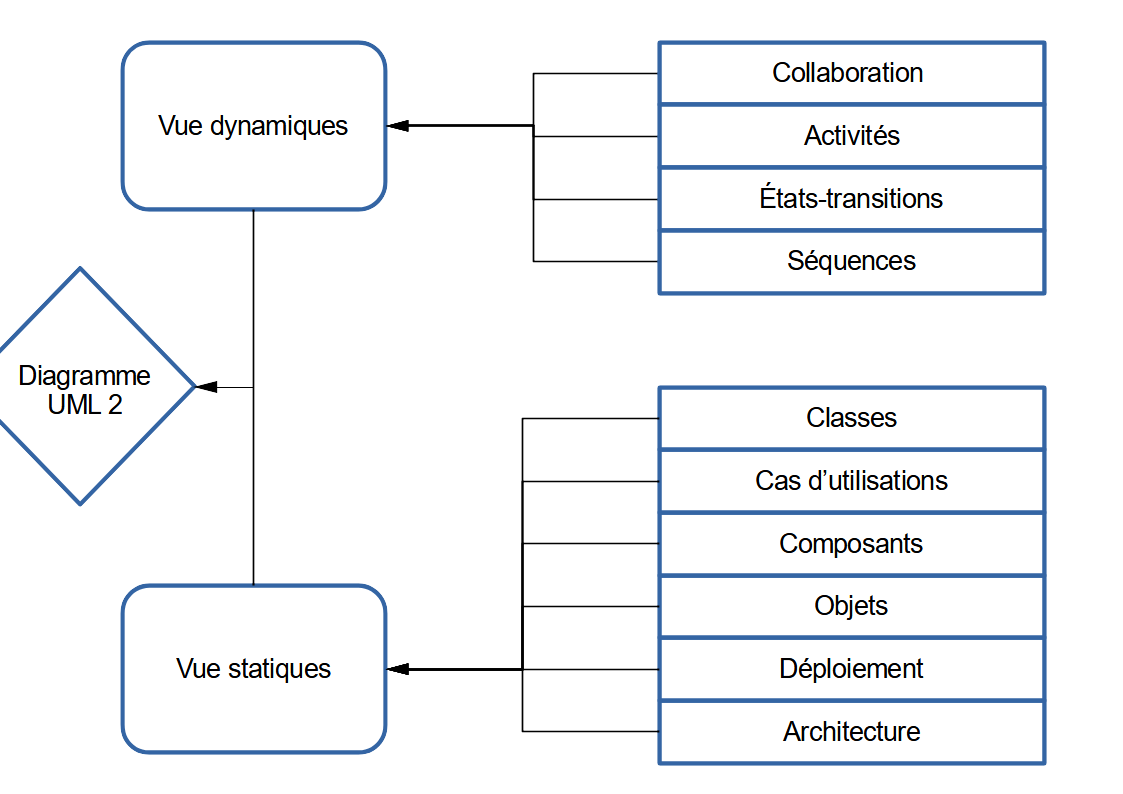
\includegraphics[height=8cm]{Figures/TypeDiagrammesUML.png}
\caption{Types de Diagrammes UML \cite{ref3}}.
\label{fig:my_label}
\end{figure}
\section{Identification des acteurs }
\par Un acteur représente un rôle d'un utilisateur qui interagit avec le
système étudié. L'utilisateur peut être un utilisateur humain, une
organisation, une machine ou un autre système externe.\cite{ref4}
\par Dans notre cas, il existe deux utilisateurs, l’utilisateur principale se
représente par les personnes qui utilisent l’application web via un navigateur
web, et qui peuvent être classifiée en trois type de personnes : des clients
qui cherchent des produits ou des services, des travailleurs qui annoncent
leurs services, et finalement des commerçants qui publient leurs produits. Ce
type d’utilisateur peut être un client, travailleur et commerçant en même
temps. Le deuxième utilisateur se représente par l’administrateur de
l’application qui peut fair la gestion des catégories et approuver ou refuser
les nouveaux produits et services
\section{Les Diagrammes des cas d'utilisation }
\par En langage UML, les diagrammes de cas d'utilisation modélisent le
comportement d'un système et permettent de capturer les exigences du système.
Les diagrammes de cas d'utilisation décrivent les fonctions générales et la
portée d'un système. Ces diagrammes identifient également les interactions
entre le système et ses acteurs. Les cas d'utilisation et les acteurs dans les
diagrammes de cas d'utilisation décrivent ce que le système fait et comment les
acteurs l'utilisent, mais ne montrent pas comment le système fonctionne en
interne.\cite{ref4}
\subsection{Diagramme global des cas d'utilisations }
\begin{figure}[H]
\centering
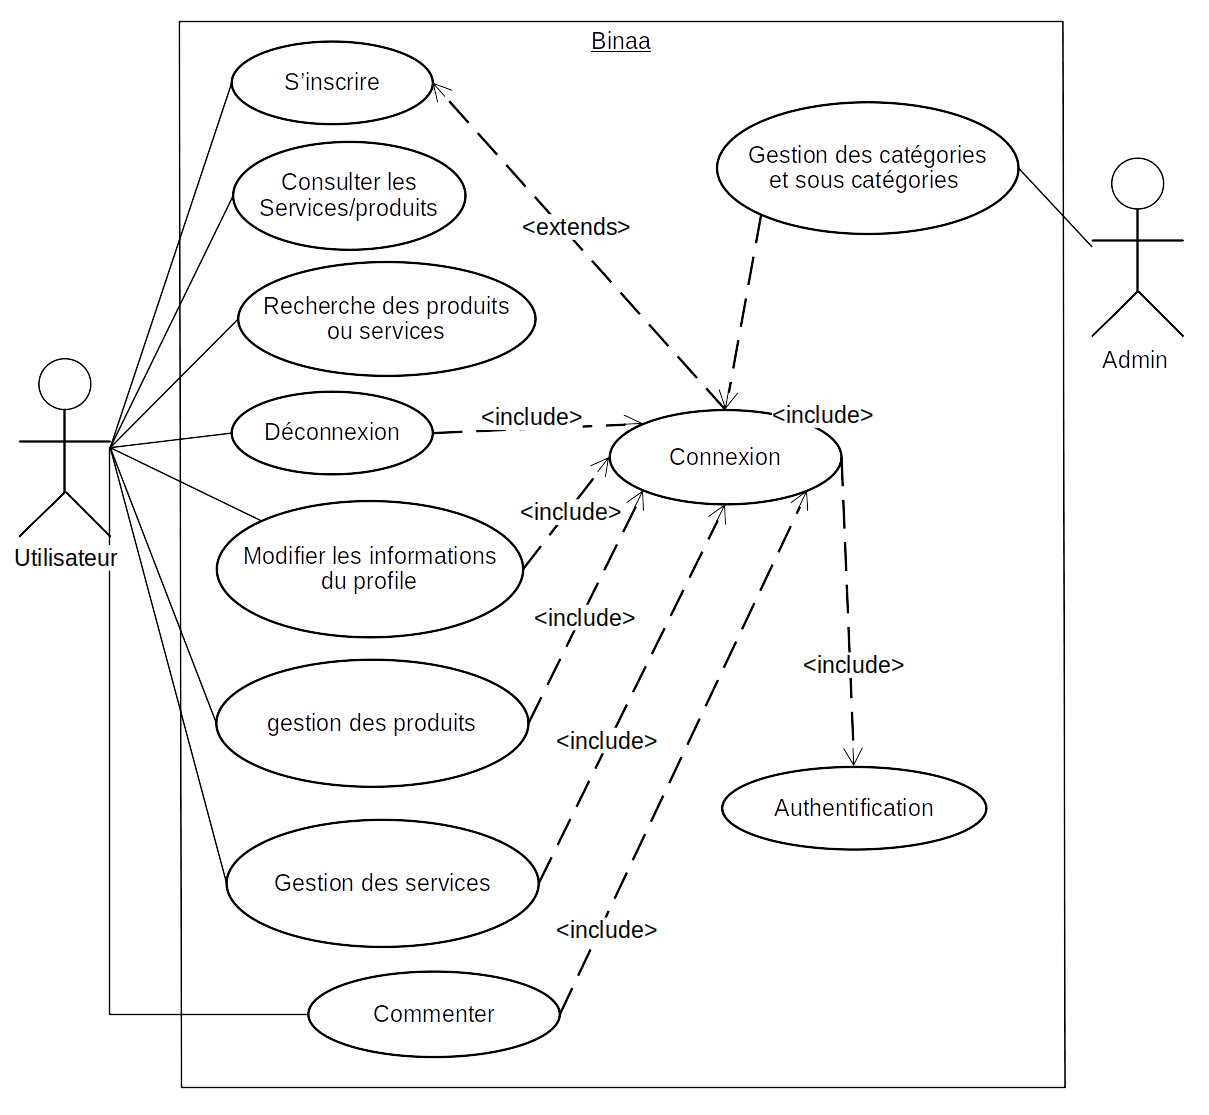
\includegraphics[scale=0.35]{images/use case/use case global.png}
\caption{Diagramme de cas d’utilisation globale}.
\label{fig:my_label}
\end{figure}
\subsection{Les différents cas d'utilisation }
\par En langage UML, les diagrammes de cas d'utilisation modélisent le
comportement d'un système et permettent de capturer les exigences du système.
Les diagrammes de cas d'utilisation décrivent les fonctions générales et la
portée d'un système. Ces diagrammes identifient également les interactions
entre le système et ses acteurs. Les cas d'utilisation et les acteurs dans les
diagrammes de cas d'utilisation décrivent ce que le système fait et comment les
acteurs l'utilisent, mais ne montrent pas comment le système fonctionne en
interne.\cite{ref4}
\par On va associer à chaque cas d’utilisation une description  textuelle des
interactions entre l’acteur et le système et les actions que le système doit
réaliser afin d’atteindre les résultats voulu par les acteurs. Pour exprimer
les cas d’utilisation de notre système, on va utiliser les formalisation
suivante :


\begin{table}[H]
\begin{tabular}{ | p{5cm} | p{10cm} |}
\hline
Numéro de cas d’utilisation & Nom de cas d’utilisation. \\ 
\hline  
But & Le but de cas d’utilisation.\\ 
\hline
Acteur & Acteur principal de cas d’utilisation. \\ \hline
Préconditions & Condition qui doit être remplie avant le début de cas
d’utilisation.  \\
\hline
Scénario nominal & Séquence d’action normales associée au cas
d’utilisation.\\
\hline
Altérnative & Séquence d’action alternative pouvant conduire également au
succès. \\
\hline
Exception & Séquence d’action conduisant à un échec. \\
\hline
\end{tabular}
\caption{Le formalisme de description des cas d'utilisation.}
\label{tab:my_label}
\end{table}



\subsection{Le cas d'utilisation Authentification }
\begin{table}[H]
\begin{tabular}{ | p{5cm} | p{10cm} |}
\hline
Cas d’utilisation N°1  & Authentification (connexion). \\ 
\hline  
But & Vérifier l'identité de l’utilisateur.\\ 
\hline
Acteur & L’utilisateur. \\ \hline
Préconditions & L’utilisateur doit avoir un compte. \\
\hline
Scénario nominal & \begin{tabular}[c]{@{}l@{}}- Demande la page
d'authentification.\\  - Le Système renvoie le formulaire
d'authentification.\\   - l’utilisateur remplit le formulaire et le valide. \\
- Le système vérifie la conformité des informations\\ saisies.(Altérnative
\textbf{A1}).\\ - Le système renvoie l’utilisateur vers la page Accueil. \\
\end{tabular}
\\
\hline
Altérnative (A1) & Dans le cas où les informations saisies sont incomplètes ou
incorrectes, le système renvoie la page d’authentification et attend que
l’utilisateur ressaisisse les informations correctement.\\
\hline
\end{tabular}
\caption{description des cas d'utilisation Authentification.}
\label{tab:my_label}
\end{table}
\subsubsection{Diagramme de cas d’utilisation Authentification}
\begin{figure}[H]
\centering
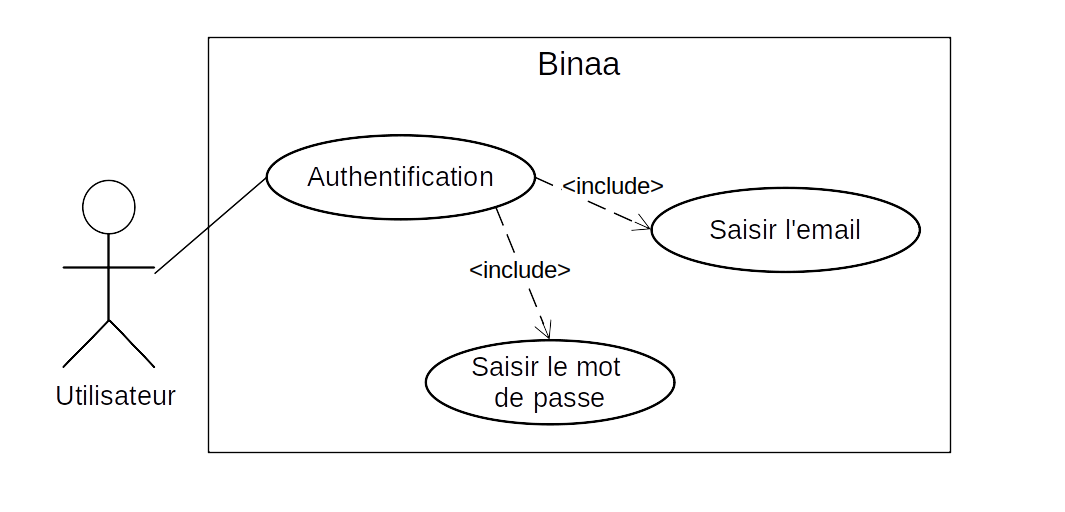
\includegraphics[scale=0.4]{images/use case/auth.png}
\caption{Diagramme du cas d'utilisation Authentificatio}.
\label{fig:my_label}
\end{figure}

\subsection{Le cas d'utilisation Inscription}
\begin{table}[H]
\begin{tabular}{ | p{5cm} | p{10cm} |}
\hline
Cas d’utilisation N°2  & Inscription. \\ 
\hline  
But & Inscrire un nouvel utilisateur.\\ 
\hline
Acteur & L’utilisateur. \\
\hline
Préconditions & Aucune. \\
\hline
Scénario nominal & \begin{tabular}[c]{@{}l@{}}- Demande du formulaire
d’inscription.\\  - Le système renvoie le formulaire d’inscription.\\   -
l’utilisateur remplit le formulaire et le valide. \\  - Le système vérifie la
conformité des informations \\ saisies.(Altérnative \textbf{A1}).\\ - Le
système renvoie l’utilisateur vers la page Accueil. \\ \end{tabular}
\\
\hline
\end{tabular}
\caption{Le formalisme de description des cas Inscription.}
\label{tab:my_label}
\end{table}
\subsubsection{Diagramme de cas d’utilisation Inscription }

\begin{figure}[H]
\centering
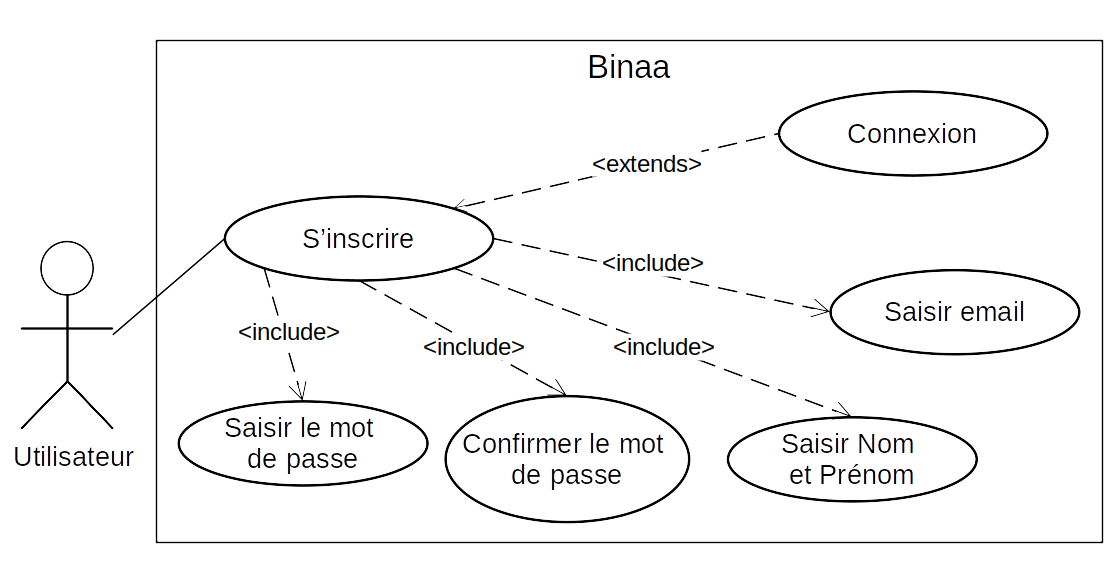
\includegraphics[scale=0.4]{images/use case/signup.png}
\caption{Diagramme du cas d'utilisation Inscription}.
\label{fig:my_label}
\end{figure}

\subsection{Le cas d'utilisation Déconnexion }
\begin{table}[H]
\begin{tabular}{ | p{5cm} | p{10cm} |}
\hline
Cas d’utilisation N°2  & Déconnexion. \\ 
\hline  
But & déconnecter l’utilisateur.\\ 
\hline
Acteur & L’utilisateur. \\
\hline
Préconditions & Authentifié. \\
\hline
Scénario nominal & \begin{tabular}[c]{@{}l@{}}- Cliquer sur le bouton
déconnexion.\\  - Renvoie à la page d’accueil.\\ \end{tabular}
\\
\hline
\end{tabular}
\caption{Le formalisme de description de cas de déconnexion.}
\label{tab:my_label}
\end{table}
\subsubsection{Diagramme du cas d'utilisation Déconnexion}

\begin{figure}[H]
\centering
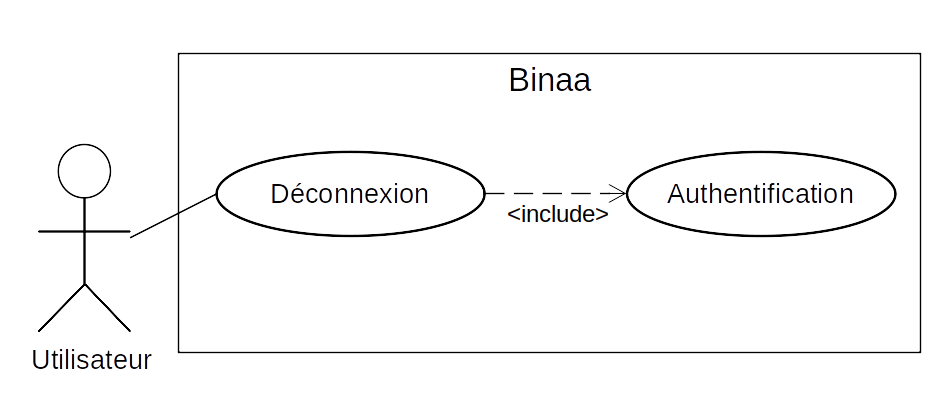
\includegraphics[scale=0.4]{images/use case/logout.png}
\caption{Diagramme du cas d'utilisation Déconnexion}.
\label{fig:my_label}
\end{figure}

\subsection{Le cas d'utilisation Gestion de profil }
\begin{table}[H]
\begin{tabular}{ | p{5cm} | p{10cm} |}
\hline
Cas d’utilisation N°2  & Gestion de profil. \\ 
\hline  
But & Modifier les informations de profil( Nom et/ou  prénom et/ou email et/ou
mot de passe).\\ 
\hline
Acteur & L’utilisateur. \\
\hline
Préconditions & Authentifié. \\
\hline
Scénario nominal & \begin{tabular}[c]{@{}l@{}}- Accéder au profil.\\  -
Demander le formulaire de modification de profil.\\   - L’utilisateur effectue
les modifications voulues et \\ valide le formulaire. \\  - Ensuit il peut y
avoir deux scenario : \\ \item a. Sans changement de mot de passe, Le système
valide \\ les modifications directement.\\ \item b. Le système effectue une
vérification de l'ancien et \\ nouveau mot de passe puis valide les
modifications (\textbf{A2})\\ \end{tabular}\\
\hline
Altérnative (A2) & Si le mot de passe est faux, le système  renvoie le
formulaire de vérification.\\
\hline
\end{tabular}
\caption{ Le formalisme de description des cas Gestion de profil.}
\label{tab:my_label}
\end{table}
\subsubsection{Diagramme de cas d’utilisation Gestion de profil}
\begin{figure}[H]
\centering
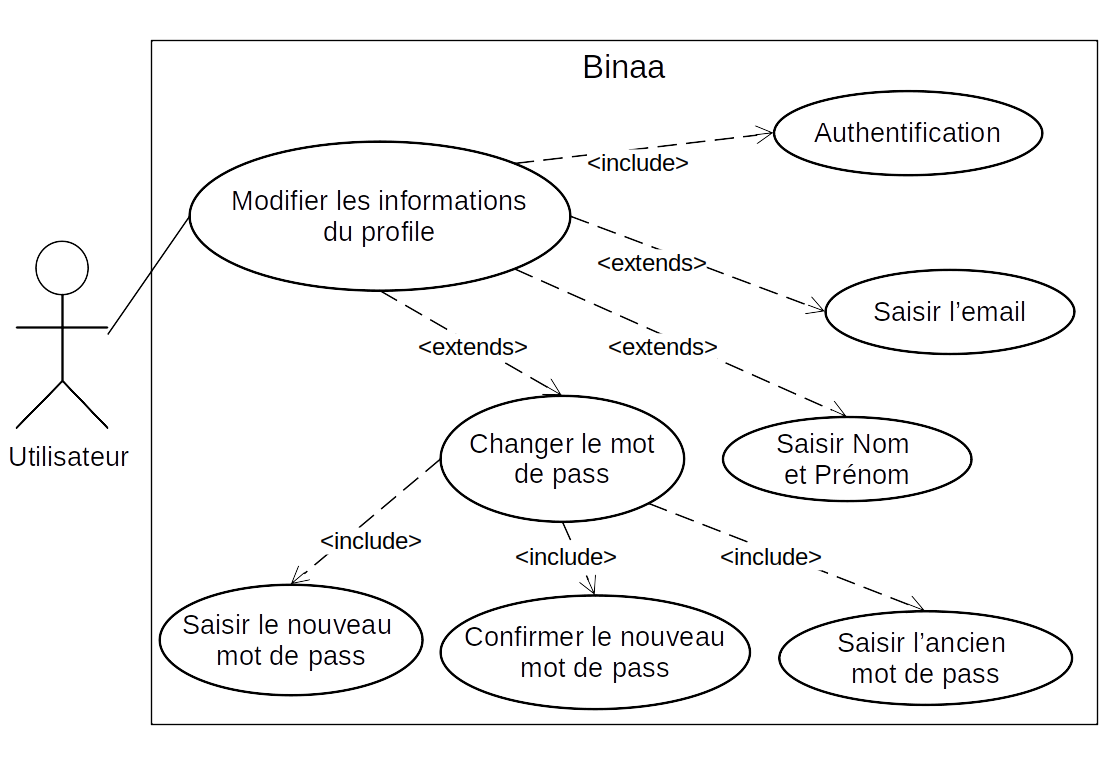
\includegraphics[scale=0.4]{images/use case/user crud.png}
\caption{Diagramme de cas d’utilisation Gestion de profil}.
\label{fig:my_label}
\end{figure}
\subsection{Le cas d'utilisation gestion de produit }
\begin{table}[H]
\begin{tabular}{ | p{5cm} | p{10cm} |}
\hline
Cas d’utilisation N°2  & Gestion de produit/service. \\ 
\hline  
But & Gestion des produits/services de l’utilisateur (ajout, modification,
suppression). \\ 
\hline
Acteur & L’utilisateur. \\
\hline
Préconditions & Authentifié. \\
\hline
Scénario nominal & \begin{tabular}[c]{@{}l@{}}- Accéder au tableaux de bord.\\
- En cas de :\\ \item a. Ajout de nouveau produit/service, l’utilisateur \\
remplit le formulaire de nouveau produit/service et \\ validé.\\ 
\item b.Sélectionner un produit/service existant pour \\ modifier ou supprimer
carrément.\\ -Le système valide la requête (soit ajout ou \\ modification ou
suppression).\\ \end{tabular}\\
\hline
Altérnative (A2) & Si le mot de passe est faux, le système  renvoie le
formulaire de vérification.\\
\hline
\end{tabular}
\caption{description des cas d'utilisation Gestion de produit/service.}
\label{tab:my_label}
\end{table}
\subsubsection{Diagramme de cas d’utilisation Gestion de produit et service}
\begin{figure}[H]
\centering
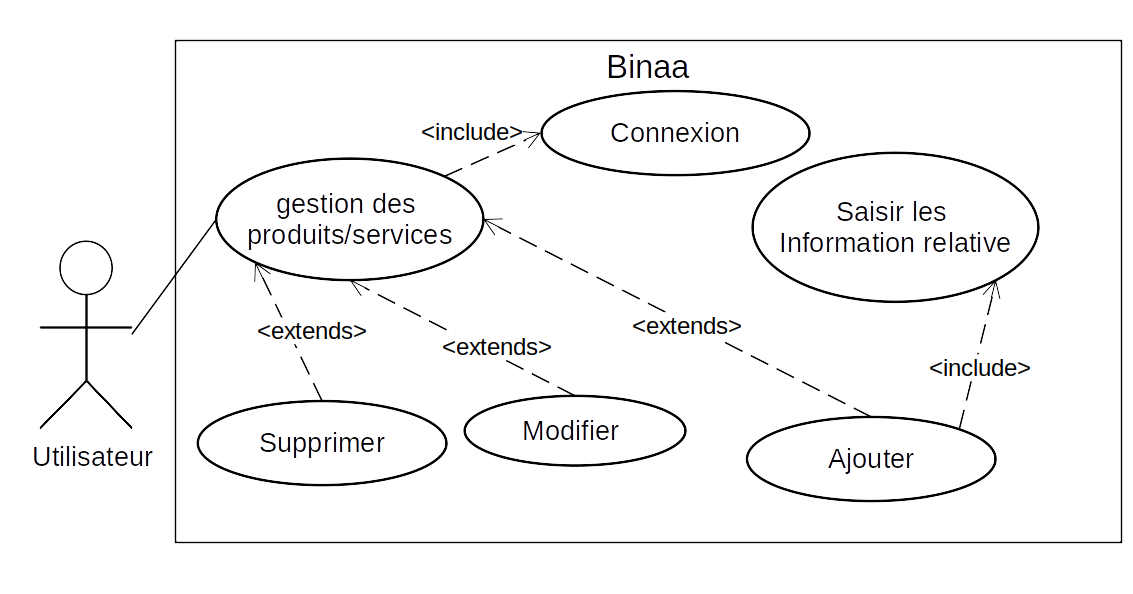
\includegraphics[scale=0.4]{images/use case/crud ps.png}
\caption{Diagramme de cas d’utilisation Gestion de produit et service}.
\label{fig:my_label}
\end{figure}
\subsection{Le cas d'utilisation donner avis }
\begin{table}[H]
\begin{tabular}{ | p{5cm} | p{10cm} |}
\hline
Cas d’utilisation N°2  & Donner avis. \\ 
\hline  
But & Donner son avis sur un produit et/ou un service.\\ 
\hline
Acteur & L’utilisateur. \\
\hline
Préconditions & Authentifié. \\
\hline
Scénario nominal & \begin{tabular}[c]{@{}l@{}}-Consulter le produit ou
service.\\  - Naviguer vers la section de commentaire .\\   - Donner une note
sur 5. \\  - Ecrire un commentaire dans le formulaire de \\ commentaire. \\
-Valider le formulaire.\\ - Le système valide le commentaire. \\ \end{tabular}
\\
\hline
\end{tabular}
\caption{description des cas d'utilisation donner avis.}
\label{tab:my_label}
\end{table}
\subsubsection{Diagramme de cas d’utilisation donner avis}
\begin{figure}[H]
\centering
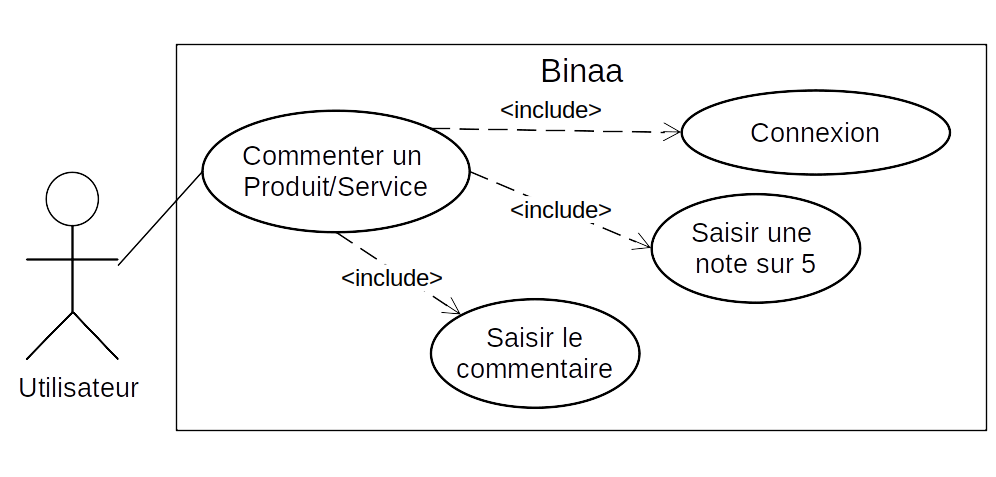
\includegraphics[scale=0.4]{images/use case/rating.png}
\caption{Diagramme du cas d'utilisation donner avis}.
\label{fig:my_label}
\end{figure}
\subsection{Le cas d'utilisation gestion de catégorie et sous-catégorie }
\begin{table}[H]
\begin{tabular}{ | p{5cm} | p{10cm} |}
\hline
Cas d’utilisation N°2  & gestion de catégorie et sous-catégorie. \\ 
\hline  
But & L’ajout, modification ou suppression d’une catégorie ou une
sous-catégorie.\\ 
\hline
Acteur & Administrateur. \\
\hline
Préconditions & Authentifié. \\
\hline
Scénario nominal & \begin{tabular}[c]{@{}l@{}}-Accéder à l’espace
administrateur.\\  - Accéder à l’espace catégorie et sous-catégorie.\\   -
Ajouter, supprimer ou modifier une catégorie ou \\ une sous-catégorie et
valider. \\  - Le système valide l’ajout, suppression ou modification. \\
\end{tabular}
\\
\hline
\end{tabular}
\caption{description des cas d'utilisation gestion de catégorie et
sous-catégorie.}
\label{tab:my_label}
\end{table}
\subsubsection{Diagramme de cas d’utilisation gestion de catégorie et
sous-catégorie }
\begin{figure}[H]
\centering
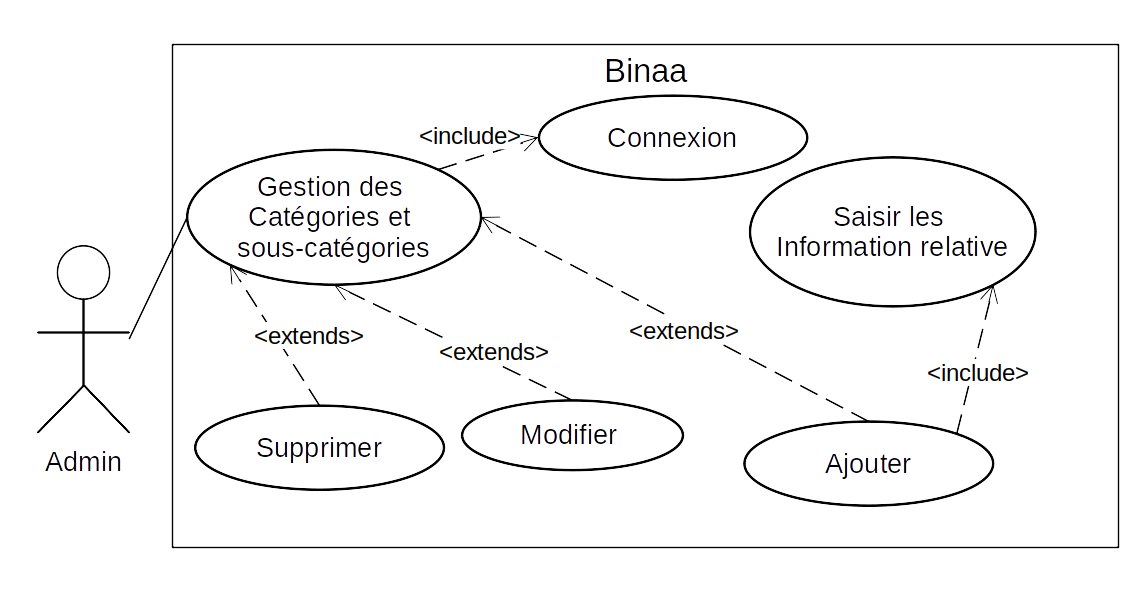
\includegraphics[scale=0.4]{images/use case/category crud.png}
\caption{Diagramme de cas d’utilisation gestion de catégorie et
sous-catégorie}.
\label{fig:my_label}
\end{figure}
\section{Diagramme de séquence }
\par Le diagramme de séquence décrit les interactions entre un groupe d'objets
en
montrant, de façon séquentielle, les envois de message qui interviennent entre
les objets. Le diagramme peut également montrer les transmissions de données
échangées lors des envois de message.\cite{ref5}

\subsection{Diagramme de séquence d'Authentification }
\begin{figure}[H]
\centering
\includegraphics[scale=0.6]{images/Diagramme de séquence/authentification
(2).png}
\caption{ Diagramme de séquence d'Authentification.}
\label{fig:my_label}
\end{figure}

\subsection{Diagramme de séquence modification de mot de passe }
\begin{figure}[H]
\centering
\includegraphics[scale=0.6]{images/Diagramme de séquence/Modification de mot de
passe (1).png}
\caption{Diagramme de séquence modification de mot de passe.}
\label{fig:my_label}
\end{figure}

\subsection{Diagramme de séquence Ajout de produit/service }
\begin{figure}[H]
\centering
\includegraphics[scale=0.6]{images/Diagramme de séquence/Ajout de
produit_service (1).png}
\caption{Diagramme de séquence Ajout de produit/service.}
\label{fig:my_label}
\end{figure}

\subsection{Diagramme de séquence donner avis }
\begin{figure}[H]
\centering
\includegraphics[scale=0.6]{images/Diagramme de séquence/Donner un avis
(1).png}
\caption{Diagramme de séquence donner avis.}
\label{fig:my_label}
\end{figure}